% Multiple Choice Question 29 to 30 (2 questions)

% \par\noindent\rule{0.75\textwidth}{0.5pt} 
\textbf{See the instruction for questions \inteval{\value{question}+1} to \inteval{\value{question}+2}.} 

\begin{center}
    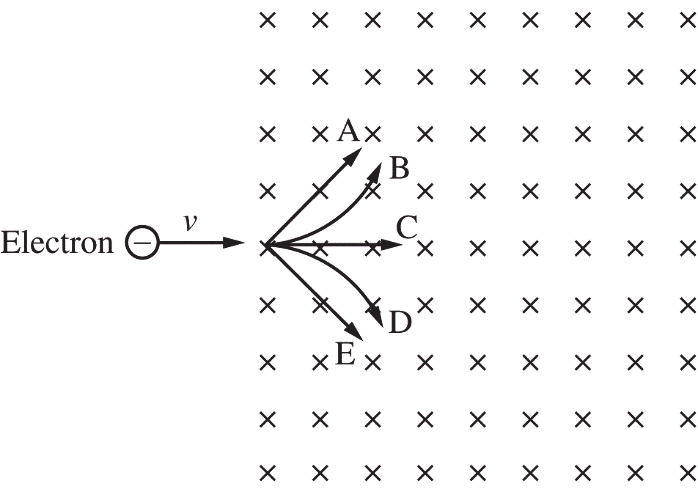
\includegraphics[scale=0.3]{images/img-014-026.png}
\end{center}

An electron is traveling with speed $v$ when it enters a uniform magnetic field that is directed into the page, as shown above. Five paths in the magnetic field are labeled A, B, C, D, E.

\begin{questions}
\setcounter{question}{28}

% Multiple Choice Question 29
\question
Which labeled path best shows the path the electron will follow as it travels through the magnetic field?

\begin{oneparchoices}
    \choice Path A
    \choice Path B
    \choice Path C
    \choice Path D
    \choice Path E
\end{oneparchoices}

% Multiple Choice Question 30

\question
The electron is replaced with a proton that is traveling at the same speed $v$ in the same direction as it enters the magnetic field. Which of the following best describes the motion of the proton as it passes through the magnetic field?

\begin{enumerate}
    \item The speed of the proton changes less than the speed of the electron did.
    \item The proton is deflected in the opposite direction.
    \item The proton is deflected more than the electron.
\end{enumerate}

\begin{oneparchoices}
    \choice I only
    \choice I and II only
    \choice II only
    \choice II and III only
    \choice I, II and III
\end{oneparchoices}

\end{questions}
